%% Part of Stellarium User Guide
%% History: 
%% 2016-04-24 Adapted from GZ's course given at SEAC2015 in Rome.
%% 2016-04-25 Added section on making Nadir image for old_style landscape.
%% State: Current for 0.15.


\chapter{Landscapes}
\label{ch:landscapes}
\chapterauthor*{Georg Zotti}

\newcommand{\landscape}[1]{\textsf{\textit{\footnotesize #1}}}

  
Landscapes are one of the key features that make Stellarium popular.
Originally just used for decoration, since version 10.6 they can be
configured accurately for research and demonstration in ``skyscape
astronomy'', a term which describes the connection of landscape and
the sky above~\cite{Brown:JSA2015}. Configured properly, they can act as reliable proxies
of the real landscapes, so that you can take e.g.\ measurements of
sunrise or stellar alignments~\cite{Zotti-Neubauer:SEAC2011}, or prepare your next moonrise
photograph, as though you were on-site.

In this chapter you can find relevant information required to
accurately configure Stellarium landscapes, using panoramas created
from photographs taken on-site, optionally supported by horizon
measurements with a theodolite.


Creating an accurate panorama requires some experience with
photography and image processing. However, great open-source tools
have been developed to help you on the job. If you already know other
tools, you should be able to easily transfer the presented concepts to
those other tools.


\section{Stellarium Landscapes}
\label{sec:landscapes:StellariumLandscapes}


As of version 0.15, the available landscape types are:
\begin{description}
\item[polygonal] A point list of measured azimuth/altitude pairs, used
  to define a sharp horizon polygon. The area below the horizon line
  is colored in a single color
  (Section~\ref{sec:landscapes:Polygonal}).
\item[spherical] The simple form to configure a photo-based panorama:
  A single image is used as texture map for the horizon
  (Section~\ref{sec:landscapes:Spherical}).
\item[old\_style] The original photo panorama. This is the most
  difficult to configure, but allows highest resolution by using
  several texture maps (Section~\ref{sec:landscapes:oldStyle}).
\item[fisheye] Another 1-texture approach, utilizing an image made
  with a fisheye lens. This landscape suffers from calibration
  uncertainties and can only be recommended for decoration
  (Section~\ref{sec:landscapes:Fisheye}).
\end{description}

A landscape consists of a \file{landscape.ini} plus the data files
that are referenced from there, like a coordinate list or the
textures. Those reside in a subdirectory of the \file{landscape}
folder inside the Stellarium program directory, or, for own work, in a
subdirectory of the \file{landscape} folder inside your Stellarium
user data directory (see section~\ref{sec:Directories}). 

Let us ssume we want to create a landscape for a place called
Rosenburg.  The location for the files of our new custom landscape
\landscape{Rosenburg} depends on the operating system (see
\ref{sec:Directories}). Create a new subdirectory, and for maximum
compatibility, use small letters and no spaces:

\noindent
\begin{tabular}{ll}
Windows&  \file{C:/Users/YOU/AppData/Roaming/Stellarium/landscapes/rosenburg}\\
Linux&\file{\textasciitilde/.stellarium/landscapes/rosenburg}\\
Mac&\file{\$HOME/Library/Preferences/Stellarium/landscapes/rosenburg}\\
\end{tabular}


% \noindent The user data directory is unfortunately hidden by default
% on all systems. (On UNIX-like systems, directories starting with a
% \file{.} are hidden.) To make it accessible in the Windows file
% explorer, open an Explorer window and select \menu{Organize..., Folder and
% search options}. Make sure folders marked as hidden are still
% displayed. Also, deselect the checkbox to hide known file name
% endings.\footnote{This is a very confusing default setting and in fact
%   a security risk: Consider you receive some file
%   \file{funny.png.exe}. Your explorer displays this as
%   \file{funny.png}. You double-click it, expecting to open some image
%   browser with a funny image. However, you start some unknown program
%   instead, and running this \file{.exe} executable program may turn
%   out to be anything but funny!}
% 

\subsection{Location information}
\label{sec:landscapes:location}

This optional section in \file{landscape.ini} allows automatic loading
of site coordinates if this option is activated in the program
GUI (see~\ref{sec:gui:view:landscape}). For our purposes we should consider especially the coordinates in
the location section mandatory!

\begin{configfile}
[location]
planet = Earth
country = Austria
name = KGA Rosenburg
latitude = +48d38'3.3"
longitude = +15d38'2.8"
altitude = 266
light_pollution = 1
atmospheric_extinction_coefficient = 0.2
display_fog = 0
atmospheric_temperature = 10.0
atmospheric_pressure = 1013.0
\end{configfile}
%
Where:
\begin{description}
\item[\var{planet}] Is the English name of the solar system body for
  the landscape.
\item[\var{latitude}] Is the latitude of site of the landscape in
  degrees, minutes and seconds. Positive values represent North of the
  equator, negative values South of the equator.
\item[\var{longitude}] Is the longitude of site of the
  landscape. Positive values represent East of the Greenwich Meridian
  on Earth (or equivalent on other bodies), Negative values represent
  Western longitude.
\item[\var{altitude}] Is the altitude of the site of the landscape in meters.
\item[\var{country}] (optional) Name of the country the location is in.
\item[\var{state}] (optional) Name of the state the location is in.
\item[\var{name}] (optional) Name of the location. This may contain
  spaces, but keep it short to have it fully visible in the
  selection box.
\end{description}
%
Since V0.11, there are a few more optional parameters that can be
loaded if the according switch is active in the landscape selection
panel. If they are missing, the parameters do not change to defaults.

\begin{description}
\item[\var{light\_pollution}] (optional) Light pollution of the site,
  given on the Bortle Scale (1: none \ldots 9: metropolitan; see
  Appendix \ref{ch:BortleScale}). If negative or absent, no change
  will be made.
\item[\var{atmospheric\_extinction\_coefficient}] (optional, no change
  if absent.) Extinction coefficient (mag/airmass) for this site.
\item[\var{atmospheric\_temperature}] (optional, no change if absent.)
  Surface air temperature (Degrees Celsius). Used for refraction. Set
  to -1000 to explicitly declare "no change".
\item[\var{atmospheric\_pressure}] (optional, no change if absent.)
  Surface air pressure (mbar; would be 1013 for "normal" sea-level
  conditions). Used for refraction. Set to -2 to declare "no change",
  or -1 to compute from altitude.
\item[\var{display\_fog}] (optional, -1/0/1, default=-1) You may want
  to preconfigure setting 0 for a landscape on the Moon. Set -1 to
  declare "no change".
\end{description}


\subsection{Polygonal landscape}
\label{sec:landscapes:Polygonal}

This landscape type has been added only recently (since 0.13) to allow
the use of measured horizons. Users of \program{Cartes du
  Ciel}\footnote{SkyChart / Cartes du Ciel planetarium:
  \url{http://www.ap-i.net/skychart/en/start}} will be happy to hear
that the format of the list of measurements is compatible.

This is the technically simplest of the landscapes, but may be used to
describe accurately measured horizon lines. The file that encodes
horizon altitudes can also be used in all other landscape types. If
present there, it will be used to define object visibility (instead of
the opacity of the landscape photo textures) and, if
\var{horizon\_line\_color} is defined, will be plotted.

There is a small caveat: Sometimes, there may appear vertical lines
from some corners towards the zenith or the mathematical horizon,
e.g.\ if there is a vertex including azimuth 0 or 180. If this
irritates you, just offset this azimuth minimally (e.g., 180.00001).

The \file{landscape.ini} file for a polygonal type landscape looks
like this (this example is based on the \landscape{Geneve} landscape
which was borrowed from Cartes du Ciel and comes with Stellarium):

\begin{configfile}
[landscape]
name = Geneve
type = polygonal
author = Georg Zotti; Horizon definition by Patrick Chevalley
description = Horizon line of Geneve. 
              Demonstrates compatibility with 
              horizon descriptions from Cartes du Ciel.
polygonal_horizon_list = horizon_Geneve.txt
polygonal_angle_rotatez = 0
ground_color = .15,.45,.45
horizon_line_color = .75,.45,.45
\end{configfile}
%
Where:
\begin{description}
\item[\var{name}] appears in the landscape tab of the configuration window.
\item[\var{type}] identifies the method used for this landscape. \var{polygonal} in this case.
\item[\var{author}] lists the author(s) responsible for images and composition.
\item[\var{description}] gives a short description visible in the
  selection panel. The text can be superseded by optional
  \file{description.<lang>.utf8} files.
\item[\var{polygonal\_horizon\_list}] is the name of the horizon data file for this landscape.
\item[\var{polygonal\_horizon\_list\_mode}] (optional) the two first
  columns in the list are numbers: azimuth and altitude or zenith
  distance, in either degrees or radians or gradians(gon). The value
  must be one of \var{azDeg\_altDeg}, \var{azDeg\_zdDeg}, \var{azRad\_altRad},
    \var{azRad\_zdRad}, \var{azGrad\_altGrad}, \var{azGrad\_zdGrad}. Default:
  \var{azDeg\_altDeg}
\item[\var{polygonal\_angle\_rotatez}] (optional, default=0) Angle
  (degrees) to adjust azimuth. This may be used to apply a (usually)
  small offset rotation, e.g. when you have measured the horizon in a
  grid-based coordinate system like UTM and have to compensate for the
  meridian convergence.
\item[\var{ground\_color}] (optional, default=\var{0,0,0}, i.e.,
  black) Color for the area below the horizon line. Each R,G,B
  component is a float within 0..1.
\item[\var{horizon\_line\_color}] (optional, default: invisible) used
  to draw a polygonal horizon line. Each R,G,B component is a float
  within 0..1.
\item[\var{minimal\_brightness}] (optional) Some minimum brightness to
  keep landscape visible. Default=-1, i.e., use
  \var{minimal\_brightness} from the \var{[landscape]} section in the
  global \file{config.ini}.
\item[\var{minimal\_altitude}] (optional, default=-2) Some sky
  elements, e.g.\ stars, are not drawn below this altitude to increase
  performance. Under certain circumstances you may want to specify
  something else here. (since V0.14)
\item[\var{polygonal\_horizon\_inverted}] (optional, default=false) In
  rare cases like horizon lines for high mountain peaks with many
  negative horizon values this should be set to true. (since V0.15)
\end{description}


\subsection{Spherical landscape}
\label{sec:landscapes:Spherical}

This method uses a more usual type of panorama -- the kind which is
produced directly from software such as \program{autostitch} or
\program{Hugin}\footnote{\url{http://hugin.sourceforge.net/}}.  The
\landscape{Moon} landscape which comes with Stellarium provides a
minimal example of a \file{landscape.ini} file for a spherical type
landscape:

\begin{configfile}
[landscape]
name = Moon
type = spherical
maptex = apollo17.png
\end{configfile}
A more elaborate example is found with the \landscape{Grossmugl} landscape: 

\begin{configfile}
[landscape]
name = Grossmugl
type = spherical
author = Guenther Wuchterl, Kuffner-Sternwarte.at; 
         Lightscape: Georg Zotti
description = Field near Leeberg, Grossmugl (Riesentumulus), 
              Austria - Primary Observing Spot of the Grossmugl 
              Starlight Oasis - http://starlightoasis.org
maptex = grossmugl_leeberg_crop11.25.png
maptex_top=11.25 
maptex_fog = grossmugl_leeberg_fog_crop22.5.png
maptex_fog_top = 22.5
maptex_fog_bottom = -22.5
maptex_illum = grossmugl_leeberg_illum_crop0.png
maptex_illum_bottom = 0
angle_rotatez=-89.1
minimal_brightness = 0.0075
polygonal_horizon_list = horizon_grossmugl.txt
polygonal_angle_rotatez=0
horizon_line_color =  .75,.45,.45
minimal_altitude = -1
\end{configfile}
Where:
\begin{description}
\item[\var{name}] appears in the landscape tab of the configuration window. This name may be translated.
\item[\var{type}] identifies the method used for this
  landscape. \var{spherical} in this case.
\item[\var{author}] lists the author(s) responsible for images and
  composition.
\item[\var{description}] gives a short description visible in the
  selection panel. The text will be superseded by optional
  \file{description.<lang>.utf8} files.
\item[\var{maptex}] is the name of the image file for this landscape.
\item[\var{maptex\_top}] (optional; default=90) is the altitude angle
  of the top edge.
\item[\var{maptex\_bottom}] (optional; default=-90) is the altitude
  angle of the bottom edge. Usually you will not require this, or else
  there will be a hole at your feet. ;-)
\item[\var{maptex\_fog}] (optional; default: no fog) is the name of
  the fog image file for this landscape.
\item[\var{maptex\_fog\_top}] (optional; default=90) is the altitude
  angle of the top edge of the fog texture. Useful to crop away parts
  of the image to conserve texture memory.
\item[\var{maptex\_fog\_bottom}] (optional; default=-90) is the
  altitude angle of the bottom edge.
\item[\var{maptex\_illum}] (optional; default: no illumination layer)
  is the name of the nocturnal illumination/light pollution image file
  for this landscape.
\item[\var{maptex\_illum\_top}] (optional; default=90) is the altitude
  angle of the top edge, if you have light pollution only close to the
  horizon.
\item[\var{maptex\_illum\_bottom}] (optional; default=-90) is the
  altitude angle of the bottom edge.
\item[\var{angle\_rotatez}] (optional, default=0) Angle (degrees) to
  adjust azimuth. If 0, the left/right edge is due east.
\item[\var{tesselate\_rows}] (optional, default=20) This is the number
  of rows for the maptex. If straight vertical edges in your landscape
  appear broken, try increasing this value, but higher values require
  more computing power. Fog and illumination textures will have a
  similar vertical resolution.
\item[\var{tesselate\_cols}] (optional, default=40) If straight
  horizontal edges in your landscape appear broken, try increasing.
\item[\var{polygonal\_horizon\_list}] (optional) is the name of the
  (measured) horizon data file for this landscape. Can be used to
  define the exact position of the horizon. If missing, the texture
  can be queried for horizon transparency (for accurate object
  rising/setting times)
\item[\var{polygonal\_horizon\_list\_mode}] (optional) see \ref{sec:landscapes:Polygonal}  % 
      % the two first columns in the list are numbers: azimuth and altitude or zenith distance, in either degrees or radians or gradians(gon). 
      % The value must be one of azDeg_altDeg|azDeg_zdDeg|azRad_altRad|azRad_zdRad|azGrad_altGrad|azGrad_zdGrad. Default: azDeg_altDeg
\item[\var{polygonal\_angle\_rotatez}] (optional, default=0) see \ref{sec:landscapes:Polygonal}  %Angle (degrees) to adjust azimuth. This may be used to apply a (usually) small offset rotation, e.g. when you have measured the horizon in a grid-based coordinate system like UTM and have to compensate for the meridian convergence.
\item[\var{horizon\_line\_color}] see \ref{sec:landscapes:Polygonal}  %(optional, default: invisible) used to draw a polygonal horizon line.
\item[\var{minimal\_brightness}]  see \ref{sec:landscapes:Polygonal}  %(optional, default=-1, i.e. use preset landscape/minimal_brightness from global config.ini) Some minimum brightness to keep landscape visible.
\item[\var{minimal\_altitude}] (optional, default=-2) Some sky
  elements, e.g.\ stars, are not drawn below this altitude for
  efficiency. Under certain circumstances (e.g.\ for space station
  panoramas where you may have sky below your feet, or for deep
  valleys/high mountains, you may want to specify something else
  here. (since V0.14)
\end{description}
%
To save texture memory, %since V0.13 
you can trim away the transparent
sky and define the angle \var{maptex\_top}. Likewise,
\var{fogtex\_top}, \var{fogtex\_bottom}, \var{maptex\_illum\_top} and
\var{maptex\_illum\_top}. You should then stretch the texture to a
full power of 2, like $4096\times1024$ (but note that some hardware is
even limited to 2048 pixels). The easiest method to create perfectly
aligned fog and illumination layers is with an image editor that
supports layers like the \program{GIMP} or \program{Photoshop}. Fog
and Light images should have black background.


\subsection{High resolution (``Old Style'')  landscape}
\label{sec:landscapes:oldStyle}

The \var{old\_style} or multiple image method works by having the
360\degree panorama of the horizon (without wasting too much texture
memory with the sky) split into a number of reasonably small
\emph{side textures}, and a separate \emph{ground texture}. This has
the advantage over the single-image method that the detail level of
the horizon can be increased without ending up with a single very
large image file, so this is usable for either very high-resolution
panoramas or for older hardware with limited capabilities. The ground
texture can be a different resolution than the side textures. Memory
usage may be more efficient because there are no unused texture parts
like the corners of the texture file in the fish-eye method. It is
even possible to repeat the horizon several times (for purely
decorative purpose). The side textures are mapped onto curved
(spherical ring or cylinder) walls
(Fig.~\ref{fig:landscapes:oldStyle}).

\begin{figure}[tb]
  \centering
   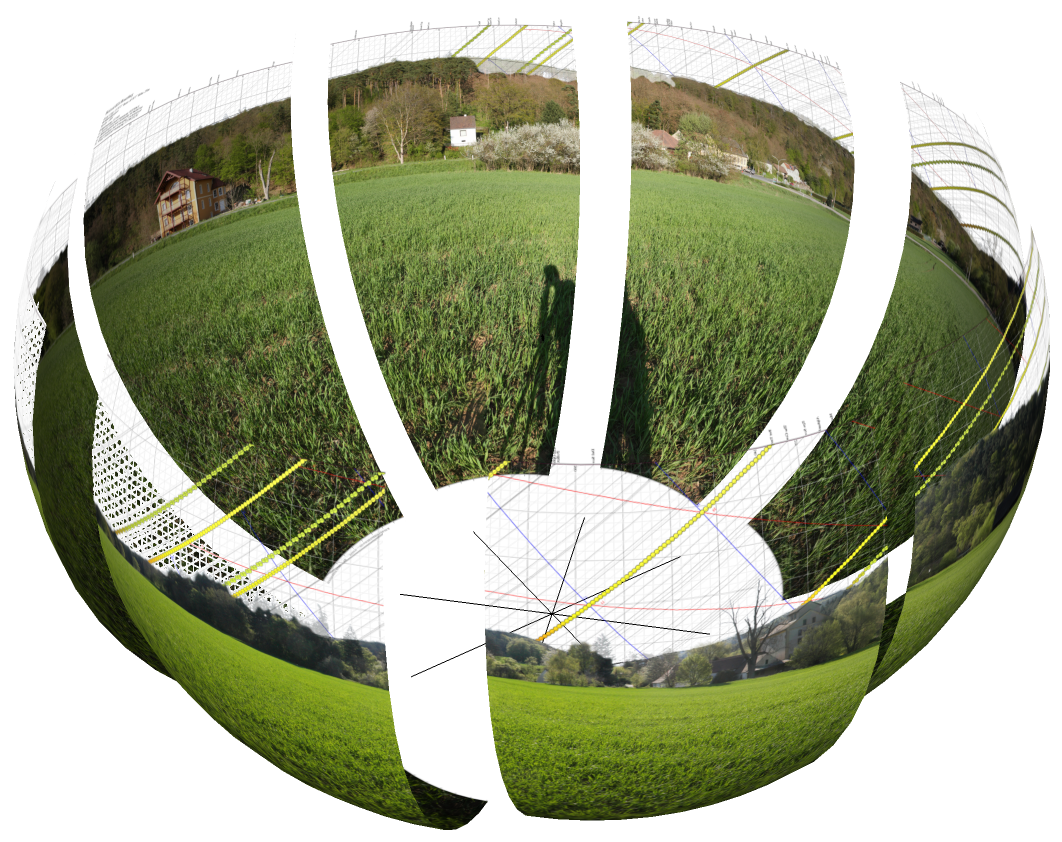
\includegraphics[width=10cm]{Rosenburg-Demo.png}
   \caption{Old\_style landscape: eight parts delivering a
     high-resolution panorama. The bottom (ground) texture, drawn on a flat
     plane, is not shown here.}
  \label{fig:landscapes:oldStyle}
\end{figure}

On the negative side, it is more difficult to create this type of
landscape -- merging the ground texture with the side textures can
prove tricky. (\program{Hugin} can be used to create also this file,
though. And on the other hand, you can replace this by something else
like a site map.) The contents of the \file{landscape.ini} file for
this landscape type is also somewhat more complicated than for other
landscape types. Here is the \file{landscape.ini} file which describes
our \landscape{Rosenburg} landscape\footnote{the \var{groundtex}
  \file{grassground.png} mentioned here has been taken from the
  \landscape{Guereins} landscape.}:

\begin{configfile}
[landscape]
name = KGA Rosenburg
author = Georg Zotti, VIAS/ASTROSIM
description = KGA Rosenburg
type = old_style
nbsidetex = 8
tex0 = Horiz-0.png
tex1 = Horiz-1.png
tex2 = Horiz-2.png
tex3 = Horiz-3.png
tex4 = Horiz-4.png
tex5 = Horiz-5.png
tex6 = Horiz-6.png
tex7 = Horiz-7.png
nbside = 8
side0 = tex0:0:0:1:1
side1 = tex1:0:0:1:1
side2 = tex2:0:0:1:1
side3 = tex3:0:0:1:1
side4 = tex4:0:0:1:1
side5 = tex5:0:0:1:1
side6 = tex6:0:0:1:1
side7 = tex7:0:0:1:1
groundtex = grassground.png
ground = groundtex:0:0:1:1
nb_decor_repeat = 1
decor_alt_angle =  82
decor_angle_shift = -62
; Rotatez deviates from -90 by the Meridian Convergence. 
; The original landscape pano is grid-aligned, not north-aligned!
decor_angle_rotatez =  -90.525837223
ground_angle_shift = -62
ground_angle_rotatez =  44.474162777
draw_ground_first = 1
fogtex = fog.png
fog_alt_angle = 20
fog_angle_shift = -3
fog = fogtex:0:0:1:1
calibrated = true
[location]
planet = Earth
latitude = +48d38'3.3"
longitude = +15d38'2.8"
altitude = 266
light_pollution = 1
atmospheric_extinction_coefficient = 0.2
display_fog = 0
atmospheric_temperature = 10.0
atmospheric_pressure = 1013.0
\end{configfile}
%
Where:
\begin{description}
\item[\var{name}] is the name that will appear in the landscape tab of the configuration window for this landscape
\item[\var{type}] should be \var{old\_style} for the multiple image method.
\item[\var{author}] lists the author(s) responsible for images and composition.
\item[\var{description}] gives a short description visible in the
  selection panel. The text will be superseded by optional
  \file{description.<lang>.utf8} files.
\item[\var{nbsidetex}] is the number of side textures for the landscape.
\item[\var{tex0 ... tex<nbsidetex-1>}] are the side texture file
  names. These should exist in the \file{textures / landscapes /
    landscape} directory in PNG format.
\item[\var{light0 ... light<nbsidetex-1>}] are optional textures. If
  they exist, they are used as overlays on top of the respective
  \var{tex<...>} files and represent nocturnal illumination,
  e.g. street lamps, lit windows, red dots on towers, sky glow by city
  light pollution, \ldots Empty (black) panels can be omitted. They
  are rendered exactly over the \var{tex<...>} files even when the PNG
  files have different size. If you need your light pollution higher in
  the sky, you must use a spherical or fisheye
  landscape.% (New feature, V0.13.1)
\item[\var{nbside}] is the number of side textures
\item[\var{side0 \ldots side<nbside-1>}] are the descriptions of how
  the side textures should be arranged in the program. Each
  description contains five fields separated by colon characters
  (\var{:}). The first field is the ID of the texture
  (e.g. \var{tex0}), the remaining fields are the texture coordinates
  (\var{x0:y0:x1:y1}) used to place the texture in the scene. If you
  want to use all of the image, this will just be \var{0:0:1:1}.
\item[\var{groundtex}] is the name of the ground texture file. (This
  could also be a diagram e.g. indicating the mountain peaks!)
%\item[\var{ground}] [NO LONGER USED] used to be the description of the projection of the ground texture in the scene.
\item[\var{fogtex}] is the name of the texture file for fog in this
  landscape. Fog is mapped onto a simple cylinder.\footnote{In very wide-angle
  views, the fog cylinder may become visible in the corners.} Note that for this
  landscape, accurate overlay of fog and landscape is only guaranteed if
  \var{calibrated=true} and \var{tan\_mode=true}. 
%\item[\var{fog}] [NO LONGER USED] used to be the description of the projection of the fog texture in the scene.
\item[\var{nb\_decor\_repeat}] is the number of times to repeat the
  side textures in the 360 panorama. (Useful photo panoramas should
  have \var{1} here)
\item[\var{decor\_alt\_angle}] (degrees) is the vertical angular
  extent of the textures (i.e. how many degrees of the full altitude
  range they span).
\item[\var{decor\_angle\_shift}] (degrees) vertical angular offset of
  the scenery textures, at which height the bottom line of the side
  textures is placed.
\item[\var{decor\_angle\_rotatez}] (degrees) angular rotation of the
  panorama around the vertical axis. This is handy for rotating the
  landscape so North is in the correct direction. Note that for
  historical reasons, a landscape with this value set to zero degrees
  has its leftmost edge pointing towards east.
\item[\var{ground\_angle\_shift}] (degrees) vertical angular offset of
  the ground texture, at which height the ground texture is placed.
\item[\var{ground\_angle\_rotatez}] (degrees) angular rotation of the
  ground texture around the vertical axis. When the sides are rotated,
  the ground texture may need to be rotated as well to match up with
  the sides.
\item[\var{fog\_alt\_angle}] (degrees) vertical angular size of the
  fog cylinder - how fog looks. Accurate vertical size requires
  \var{calibrated=true}.
\item[\var{fog\_angle\_shift}] (degrees) vertical angular offset of
  the fog texture - at what height is it drawn. Accurate vertical
  placement requires \var{calibrated=true}.
\item[\var{draw\_ground\_first}] if 1 the ground is drawn in front of
  the scenery, i.e. the side textures will overlap over the ground
  texture.
\item[\var{calibrated}] (optional). New since V0.10.6: Only if true,
  \var{decor\_alt\_angle} etc. really work as documented above. The
  (buggy) old code was left to work with the landscapes already
  existing. Note that with ``uncalibrated'' landscapes, sunrise
  computations and similar functionality which requires an accurate
  horizon line will not work.
\item[\var{tan\_mode}] (optional, not used in this file). If true, the
  panorama image must be in in cylindrical, not equirectangular
  projection. Finding \var{decor\_alt\_angle} and
  \var{decor\_angle\_shift} may be a bit more difficult with this, but
  now (V0.13) works also with calibrated. A fog image created as
  overlay on the pano will be perfectly placed.
\item[\var{decor\_angle\_rotatez}] angular rotation of the scenery
  around the vertical axis. This is handy for rotating the landscape
  so North is in the correct direction. If 0, the left edge of
  \var{tex0} is due east.
\item[\var{ground\_angle\_shift}] vertical angular offset of the
  ground texture, at which height the ground texture is placed. Values
  above -10 are not recommended for non-photographic content (e.g., a
  map) due to high distortion.
\item[\var{ground\_angle\_rotatez}] angular rotation of the ground
  texture around the vertical axis. When the sides are rotated, the
  ground texture may need to be rotated as well to match up with the
  sides. If 0, east is up. if North is up in your image, set this to
  90. Note that adjustments of \var{decor\_angle\_rotatez} require
  adjustments of this angle in the opposite direction!
\item[\var{fog\_alt\_angle}] vertical angular size of the fog cylinder.
\item[\var{fog\_angle\_shift}] vertical angular offset of the fog cylinder.
\item[\var{draw\_ground\_first}] if 1, the ground is drawn before the
  sides, i.e.\ the side textures may overlap the ground texture if
  \var{ground\_angle\_shift} > \var{decor\_angle\_shift}.
\item[\var{polygonal\_horizon\_list}] (optional) see \ref{sec:landscapes:Polygonal} %is the name of the (measured) horizon data file for this landscape. Can be used to query horizon transparency (for accurate object rising/setting times)
\item[\var{polygonal\_horizon\_list\_mode}] (optional) see \ref{sec:landscapes:Polygonal}  %the two first columns in the list are numbers: azimuth and altitude or zenith distance, in either degrees or radians or gradians(gon). The value must be one of azDeg_altDeg|azDeg_zdDeg|azRad_altRad|azRad_zdRad|azGrad_altGrad|azGrad_zdGrad. Default: azDeg_altDeg
\item[\var{polygonal\_angle\_rotatez}] (optional, default=0) see \ref{sec:landscapes:Polygonal} %Angle (degrees) to adjust azimuth. This may be used to apply a (usually) small offset rotation, e.g. when you have measured the horizon in a grid-based coordinate system like UTM and have to compensate for the meridian convergence.
\item[\var{horizon\_line\_color}] see \ref{sec:landscapes:Polygonal}  % (optional, default: invisible) used to draw a polygonal horizon line.
\item[\var{minimal\_brightness}]  see \ref{sec:landscapes:Polygonal} % (optional, default=-1, i.e. use landscape/minimal\_brightness from global config.ini) Some minimum brightness to keep landscape visible.
\item[\var{minimal\_altitude}] see \ref{sec:landscapes:Polygonal}  % (optional, default=-2) Some sky elements, e.g. stars, are not drawn below this altitude. Under certain circumstances you may want to specify something else here. (since V0.14) 
\end{description}


\subsection{Fisheye landscape}
\label{sec:landscapes:Fisheye}

The \landscape{Trees} landscape that is provided with Stellarium is an
example of the single fish-eye method, and provides a good
illustration. The centre of the image is the spot directly above the
observer (the zenith). The point below the observer (the nadir)
becomes a circle that just touches the edges of the image. The
remaining areas of the image (the corners outside the circle) are not
used.

\begin{figure}[t]
\centering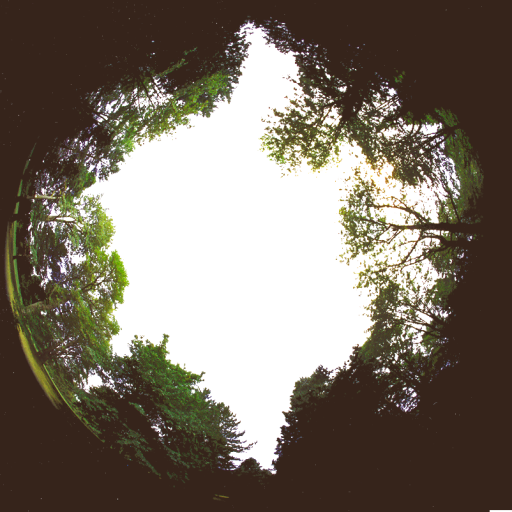
\includegraphics[width=\textwidth]{trees_512}
\caption{Texture for the \landscape{Trees} Fisheye landscape.}
\label{fig:landscapes:Fisheye}
\end{figure}


The image file (Fig.~\ref{fig:landscapes:Fisheye}) should be saved in
PNG format with alpha transparency. Whereever the image is transparent
Stellarium will render the sky.

The \file{landscape.ini} file for a fish-eye type landscape looks like
this (this example is based on the \landscape{Trees} landscape which
comes with Stellarium):

\begin{configfile}
[landscape]
name = Trees
type = fisheye
author = Robert Spearman. Light pollution image: Georg Zotti
description = Trees in Greenlake Park, Seattle
maptex = trees_512.png
maptex_illum = trees_illum_512.png
maptex_fog = trees_fog_512.png
texturefov = 210
angle_rotatez = 17
tesselate_rows = 28
tesselate_cols = 60
\end{configfile}
Where:
\begin{description}
\item[\var{name}] appears in the landscape tab of the configuration window.
\item[\var{type}] identifies the method used for this landscape. \var{fisheye} in this case.
\item[\var{author}] lists the author(s) responsible for images and composition.
\item[\var{description}] gives a short description visible in the
  selection panel. The text will be superseded by optional
  \file{description.<lang>.utf8} files.
\item[\var{maptex}] is the name of the image file for this landscape.
\item[\var{maptex\_fog}] (optional) is the name of the fog image file for this landscape.
\item[\var{maptex\_illum}] (optional) is the name of the nocturnal
  illumination/light pollution image file for this landscape.
\item[\var{texturefov}] is the field of view that the image covers in degrees.
\item[\var{angle\_rotatez}] (optional) Angle (degrees) to adjust azimuth.
\item[\var{tesselate\_rows}] (optional, default=20) If straight edges
  in your landscape appear broken, try increasing.
\item[\var{tesselate\_cols}] (optional, default=40) If straight edges
  in your landscape appear broken, try increasing.
\item[\var{polygonal\_horizon\_list}] (optional) see \ref{sec:landscapes:Polygonal}  %is the name of the (measured) horizon data file for this landscape.
\item[\var{polygonal\_horizon\_list\_mode}] (optional) see \ref{sec:landscapes:Polygonal} 
%
%  the two first columns in the list are numbers: azimuth and altitude or zenith distance, in either degrees or radians or
%  gradians(gon). The value must be one of \var{azDeg\_altDeg | azDeg\_zdDeg | azRad\_altRad | azRad\_zdRad | azGrad\_altGrad |  azGrad\_zdGrad}. Default: \var{azDeg\_altDeg}
%
\item[\var{polygonal\_angle\_rotatez}] (optional, default=0) see \ref{sec:landscapes:Polygonal} % Angle (degrees) to adjust azimuth. This may be used to apply a (usually) small offset rotation, e.g.\ when you have measured the horizon in a grid-based coordinate system like UTM and have to compensate for the meridian convergence.
\item[\var{horizon\_line\_color}] see \ref{sec:landscapes:Polygonal} % (optional, default: invisible) used to draw a polygonal horizon line.
\item[\var{minimal\_brightness}]  see \ref{sec:landscapes:Polygonal} % (optional, default=-1, i.e. use preset \var{landscape/minimal\_brightness} from global \file{config.ini}) Some minimum brightness to keep landscape visible.
\item[\var{minimal\_altitude}] see \ref{sec:landscapes:Polygonal} % (optional, default=-2) Some sky elements, e.g. stars, are not drawn below this altitude. Under certain circumstances you may want to specify something else here. (since V0.14) 
\end{description}


\subsection{Description}
\label{sec:landscapes:Description}

The short \var{description} entry in \file{landscape.ini} will be
replaced by the contents of an optional file
\file{description.<LANG>.utf8}. \file{<LANG>} is the ISO~639-1
language code, or its extension which contains language and country
code, like \file{pt\_BR} for Brazilian Portuguese. The long
description requires the file \file{description.en.utf8}, this is
\texttt{en=english} text with optional HTML tags for sections, tables,
etc. You can also have embedded images in the HTML (Views of sacred
landscapes, other informative images, \ldots?), just make them PNG
format please. The length of the description texts is not limited, you
have room for a good description, links to external resources,
whatever seems suitable.

If you can provide other languages supported by Stellarium, you can
provide translations yourself, else Stellarium translators \emph{may}
translate the English version for you. (It may take years though.) The file
ending \file{.utf8} indicates that for special characters like ÄÖÜßáé
you should use UTF8 encoding. If you write only English/ASCII, this may not
be relevant.



\subsection{Gazetteer}
\label{sec:landscapes:Gazetteer}

\newFeature{0.14}
An optional feature for landscapes is a gazetteer function, i.e., labels for
landscape features. The \landscape{Grossmugl} landscape demonstrates
an example and should be self-explanatory. This is again multilingual,
so the files are called \file{gazetteer.<LANG>.utf8}.

\begin{configfile}[\scriptsize]
# demo gazetteer for Grossmugl landscape.
# Can be used to better describe the landscape, 
# i.e. show labels on landscape features.
# Fields must be separated by vertical line, 
# label must not have such a vertical line.
# Comments have this hash mark in first column. 
# coordinates in degrees from true North. 
# line towards zenith draws a single line strictly upward.
# label is centered on line endpoint. 
# Azimuth | Altitude | degrees        | azimuth | label
#         |          | towards zenith |  shift  |               
113.66    | 5.5      |     4          |   -6    | Leeberg
35        | 1.5      |     2.5        |    0    | Grossmugl
335       | 2        |     2          |    0    | Steinabrunn
305       | 2        |     1          |    0    | Ringendorf
180       | 2        |     2          |    0    | Vienna (30km)
135       | 2        |     0.5        |    0    | Wind power plant Strasshof
\end{configfile}


\newpage

\section{Creating Panorama Photographs for Stellarium}
\label{sec:landscapes:PanoramaPhotography}

\subsection{Panorama Photography}
\label{sec:landscapes:PanoramaPhotography:Photography}

Traditional film-based panorama photography required dedicated cameras with curved
film holders and specialized lenses
(Figure~\ref{fig:landscapes:panoCam}).


\begin{figure}[tbp]
  \centering
 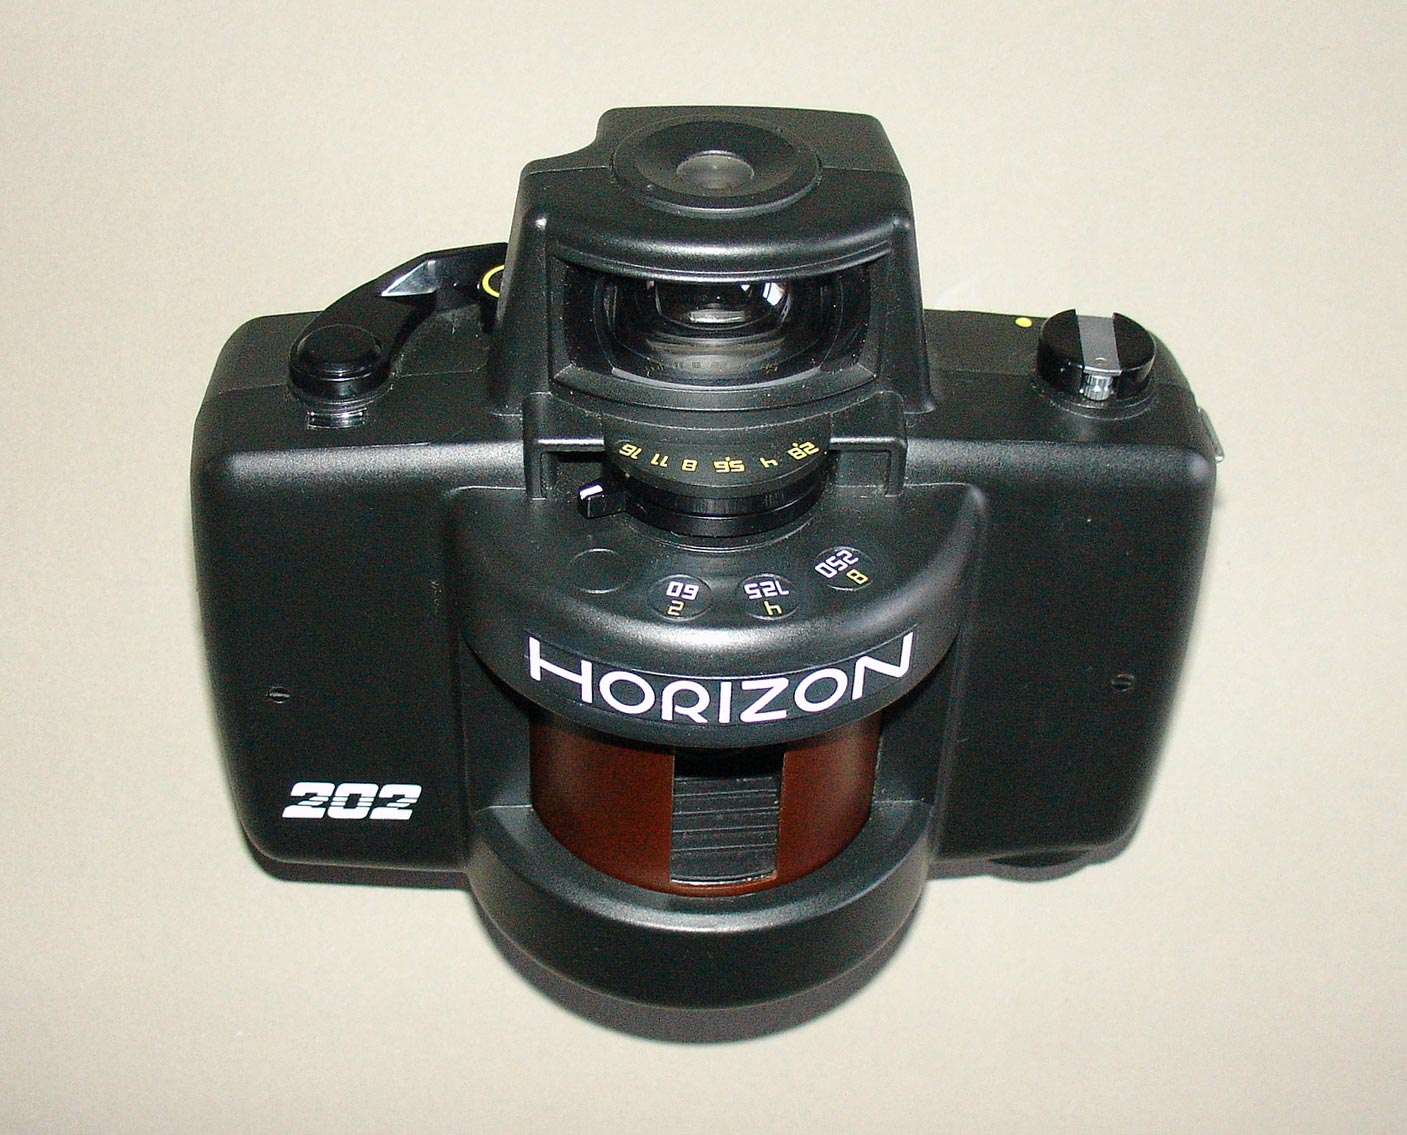
\includegraphics[width=9cm]{Horizon202.jpg}
 \caption{Zenit ``Horizon 202'' panorama camera with rotating lens for
   35mm film. \footnotesize{(Source: Wikipedia, ``Horizon202'' by
     BillC - Own Work. Licensed under CC BY-SA 3.0 via Wikimedia
     Commons -
     \url{https://commons.wikimedia.org/wiki/File:Horizon202.jpg\#mediaviewer/File:Horizon202.jpg})}}
  \label{fig:landscapes:panoCam}
\end{figure}



\begin{figure}[tbp]
  \centering
  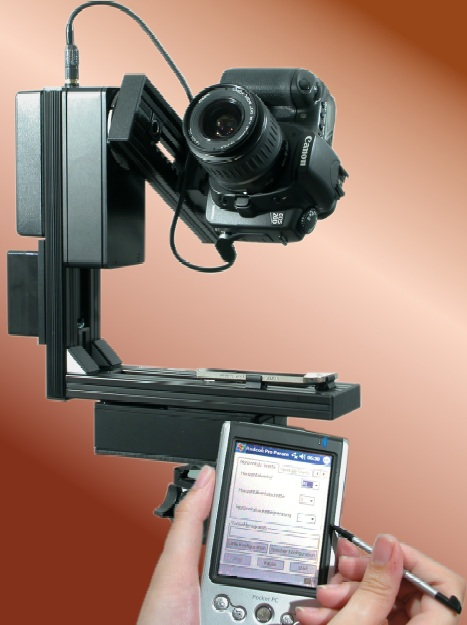
\includegraphics[width=7cm]{Rodeon_vr_head_01.jpg}
  \caption{Automated panorama head. \footnotesize{(Source: Wikipedia \url{https://de.wikipedia.org/wiki/Panoramakamera\#mediaviewer/File:Rodeon_vr_head_01.jpg})}}
  \label{fig:landscapes:panoHead}
\end{figure}


Digital photography has brought a revolution also in this field, and it has
become quite easy to create panoramas simply by taking a series of
photographs with a regular camera on the same spot and combining them
with dedicated software.

A complete panorama photo visually encloses the observer like the
mental image that astronomers have been using for millennia: the
celestial sphere. If we want to document the view, say, in a big hall
like a church, optimal results will be gained with a camera on a
tripod with a specialized panorama head (Figure~\ref{fig:landscapes:panoHead}) which assures the camera
rotates around the \emph{entrance pupil}\footnote{In many references
  you will find ``Nodal Point'' mentioned here. But see these:
  \url{http://en.wikipedia.org/wiki/Cardinal_point_\%28optics\%29\#Nodal_points},
  \url{http://web.archive.org/web/20060513074042/http://doug.kerr.home.att.net/pumpkin/Pivot_Point.pdf},
  \url{http://www.janrik.net/PanoPostings/NoParallaxPoint/TheoryOfTheNoParallaxPoint.pdf}
} of the lens in order to avoid errors by the parallax shift observed
on photographs taken on adjacent but separate positions.


Often however, both the upper half of the observer's environment (the
sky) and the ground the photographer is standing on, are regarded of
lesser importance, and only a series of laterally adjacent photographs
is taken and combined into a cylindrical or spherical ring that shows 
the landscape horizon, i.e.,  where ground and sky meet. If the
closest object of interest is farther away that a few metres,
requirements on parallax avoidance are far less critical, and the author
has taken lots of landscape panoramas with a camera on the usual
tripod screw, and even more entirely without a tripod. However, any visible errors
that are caused by a shifted camera will require more effort in
postprocessing.

When you have no tripod, note that \emph{you must not rotate the
  camera on your outstretched arm!} Rather, the camera's entrance
pupil must be rotated, so you should appear to dance around the
camera!

The images should match in brightness and white balance. If you can
shoot in RAW, do so to be able to change white balance later. If the
camera can only create JPG, ensure you have set the camera to a suitable white balance
before taking the photos and not to ``auto'', because this may find different settings and
thus give colour mismatches. Exposure brightness differences can be
largely removed during stitching, but good, well-exposed original
shots always give better results.

As a general recommendation, the images of a panorama should be taken
from left to right, else please accordingly invert some of the
instructions given below.

There are several panorama making programs. Often they are included in
the software that comes with a digital camera and allow the creation
of simple panoramas. Other software titles are available for
purchase. However, there is one cost-free open-source program
that does everything we need for our task, and much more:


\subsection{Hugin Panorama Software}
\label{sec:landscapes:Hugin}

\program{Hugin}\footnote{\url{http://hugin.sourceforge.net/}}, named
after one of the ravens that sits on Odin's shoulder and tells him
about the world, is a user-friendly catch-all package with graphical
user interface that allows creating panoramas with a single
application. Actually, \program{Hugin} is a GUI application which
calls several specialized sub-programs with fitting parameters.  The
instructions are based on \program{Hugin V2014.0} and
\program{2015.0}.

Typically digital images come in JPG format with information about
camera, lens, and settings stored in invisible metadata in the EXIF
format. When \program{Hugin} reads such images, it can automatically derive
focal length, field of view, and exposure differences (exposure time,
aperture, color balance) to create panoramas as easily as
possible. 

After starting \program{Hugin} for the first time, select \menu{Interface > Expert} to release several
options not visible to ``beginners''.  In the Preferences dialog
(\menu{Files > Preferences}), edit number of CPU to match the number of
cores in your computer and allow parallel processing. E.g., if you
have an Intel Core-i7, you usually can set up to 8 cores (4 cores with
hyperthreading; but maybe leave one core for your other tasks while
you wait for a processing job?).  If your PC is equipped with a
modern programmable graphics card, you can enable its use in the \menu{Programs} tab
with activating ``Use GPU for remapping''.

After that, we are ready for creating our panoramas.


\subsection{Regular creation of panoramas}
\label{sec:landscapes:Hugin:regular}

The graphical user interface (GUI) consists of a main menu, symbols, and 4 tabs. We start on the tab Photos. 
\begin{itemize}
\item \button{Add images\ldots} Opens a file browser. Select the images which you
  want to stitch. Usually, lens data (focal length, field of view,
  \ldots) are read from the EXIF data. If those are not available
  (e.g. cheap cameras, images scanned from film), you can enter those
  data on loading or later.  The images are now listed in the file
  list, and you can edit image parameters by marking one or more, and
  then choosing from the context menu which you get from pressing the
  right mouse button. In case you have used different lenses (or
  inadvertently used different focal lengths of a zoom lens), you can
  assign separate lenses to the images.

  Caveat: If you have resized the images, or produced copied on your
  RAW converter with non-native resolution, the Field of View (FoV) in
  \program{Hugin} may be misidentified. You must edit lens parameters and fill
  in the field of view from a full-size image. Else the first round of
  optimisation will run into unsolvable trouble. 
 
\item Select one image as \emph{position anchor} (usually the center
  image), and one as \emph{exposure anchor} (this can be the same
  image). For our purpose, \emph{the anchor image should face
    south}. 
  %In the concrete example of the Rosenburg data set, the
  %Rosenburg Castle is our landmark to the south, so any image that has
  %the castle close to center is a good choice for position anchor.
\item Next, we must find common feature points. The next field below
  provides the required settings. It is recommended to use the \program{CPFind}
  command. To avoid finding control points in (moving) clouds, select
  setting \button{Hugin's CPFind + Celeste}\footnote{If you forget this,
    you can remove cloud points by calling \program{Celeste} in the control
    point editor later}. Then press \button{Create control points}. This
  opens a dialog box in which you can see output of the selected
  feature point extractor. It should finish with a box telling you the
  number of identified points. In rare cases some images cannot be
  linked to others, you will have to manually add or edit feature
  points in those cases.
\item Now it's time to start optimisations. On the \menu{Geometric
  Optimimisation} combo, start with the button \button{Positions, incremental from
  anchor}, and press \button{Calculate}. Moments later, a first rough
  match is available for inspection.
\item First open the Preview window (press \keys{Ctrl+P} or click the blue icon). Assumed
  your images cover the full horizon, the window shows an
  equirectangular area (360 degrees along the horizon and 180 degrees
  from zenith to nadir). The anchor image should be close to the image
  center, and the other images should be already well-aligned to both
  sides. You can set the exact center point by clicking it in the
  image. If the horizon appears badly warped, use the right mouse key and
  click on the horizon roughly near $-90$ or $+90$ degrees (halfway to
  the left or right).
\item Open the OpenGL preview window (press \keys{Ctrl+Shift+P} or click the blue icon
  with GL inside). This panel provides several important views:
  \begin{itemize}
  \item The \menu{Preview} tab is similar to the non-OpenGL preview. You can
    display an overlay of the control points, which are colored
    according to match quality. Also, with button \button{Identify}
    activated, you see the overlapping image frames when you move the
    mouse over the image.
  \item The \menu{Layout} tab helps finding links between images.
  \item The \menu{Move/Drag} dialog may help to interactively adjust a
    panorama.
  \end{itemize}
  Sometimes the preview image may however be distorted and unusable. 
\item Open the \emph{Control Points Table} dialog (press \key{F3} or click the ``table''
  button). Here you see the points listed which link two
  images. Clicking a column label sorts by this column. It is
  recommended that only neighboring overlapping images should be
  included here. If you have very large overlap, it is possible that
  points are found between two images which are not directly
  adjacent. In the OpenGL preview window, you can use the \menu{Preview} or
  the \menu{Layout} tabs to identify those image pairs. Such points should be
  deleted. In the point table, click on columns ``Right Img.'', then
  ``Left Img.'', and then find pairs like 0/2, 1/3, 2/4 etc. Mark
  those lines, and delete the points.
\item To re-run the optimisation, press the double-arrow icon or the
  \button{calculate} button in the Optimise/Geometric area.
\end{itemize}


\subsubsection{Preliminary Geometric Optimisation}
\label{sec:landscapes:Optimisation}


Now the (usually) longest part begins: Iterative optimisation of the
photo matchpoints. If your images were taken on a panorama tripod
head, there should only be very few bad matchpoints, e.g.\ those found
on persons or clouds\footnote{You should have created control points
  with the \program{Celeste} option!} which have moved between
photos. For handheld photos, the following considerations should be
observed.

The most important line which we want to create in all perfection is the visible
horizon, where sky and earth meet. The foreground, usually grassy or
rocky, is of lesser interest, and stitching errors in those areas may
not even be relevant.

Therefore, matchpoints with large errors in the foreground can be
safely removed, while, if necessary, points on the horizon should be
added manually. Use the \menu{Control Points} tab, select adjacent
images (start with 0 on the left and 1 on the right side), and delete
the worst-fitting matchpoints closest to the camera (near the bottom
of the images). We now start a long phase of re-optimizing and
deletion of ill-matching points as long as those are far from the
horizon. When all near matchpoints are deleted, the result should
already look not too bad.

For continued optimisation, the number of parameters to optimize can
be extended. To begin, I recommend \button{Positions and View (y, p,
  r, v)}, which may find a new focal length slightly different from
the data in the EXIF tags. Again, delete further foreground points. If
after a few rounds you still have bad point distances, try
\button{Positions and Barrel Distortion (y, p, r, b)} to balance
distortion by bad optics, or even go up to \button{Everything without
  translation}.  Optimisation can only reach perfect results if you
did not move between exposures. Else, find a solution which shows the
least error.

In case you took your photos not on a tripod and moved too much, you
may even want to play with the translation options, but errors will be
increasingly hard to avoid.

\paragraph{Using Straight Edges as Guides}
If the panorama contains straight lines like vertical edges of
buildings, these can be used to automatically get a correctly levelled
horizon: Vertical lines are mapped to vertical lines in
equirectangular panos! In the \menu{Control Points} tab, select the image
with the vertical edge in both subframes, and mark points on the
vertical edge. (switch off auto-estimate!). 
Likewise, horizontal lines may help, but make sure lines like rooves
are perpendicular to your line of view, else the perspective effect
causes an inclination.

\paragraph{Multi-ring Panoramas}
If you are trying to create a panorama with several rings (horizon,
one or two rings below, and nadir area), you must try to create/keep control
points that best give a result without visible seams. In this case,
and esp.\ if you have only used a regular tripod or even dared to go
for a free-handed panorama, you may observe that it is best to remove
control points in neighboring photos in the lower rings, but keep only
the ``vertical'' links between images with similar azimuth.

In total, and if the foreground is not important but only grassy or
sandy, the rule of thumb is that the horizon images must be strongly
linked with good quality (small errors), while images in the lower
rings should be linked mostly to their respective upper photos, but
not necessarily to the  images to its sides. The resulting panorama will then
show a good horizon line, while stitching artifacts in a grassy or
otherwise only decorative ground will usually be acceptable and can,
if needed, be camouflaged in postprocessing.

This optimisation and editing of control points is likely a longish
iterative process, and these are the late night hours where you will
finally wish you had used a panorama head\ldots



\subsubsection{Masking}
\label{sec:landscapes:Masking}

If you have images with overlapping areas, you can usually not force
\program{Hugin} to take pixels from the image which you find best. you can
however mask off an area from an image which you don't want to see in
the output under any circumstances, e.g.\ a person's arm or foot in
one image. Just open the image in the \menu{Mask} tab and either press
\button{Add new mask} and draw the mask polygon covering the unwanted
area, or use the crop settings to define rectangular areas to use.

\subsubsection{Exposure disbalance}
\label{sec:landscapes:Exposure}
In the \menu{Photos} tab, select \button{Photometric parameters} on the right
side. The EV column lists the \emph{Exposure Value}. If you see disbalance
here and in the preview window, you can run a photometric optimisation
with the lowest button on the \menu{Photos} tab. Simply select Low dynamic
range and press \button{Calculate}. The preview should now show a seamless
image. If all else fails, you can edit the EV values directly. 

Advanced photographers may want to correct exposures in their RAW
images before creating JPG or TIF images to combine with
\program{Hugin}. This unfortunately may create exposure disbalance
because the EXIF tags may not be adjusted accordingly, so based on
different exposure/f-stop conbinations \program{Hugin} may think it
has to re-balance the values. In these cases, don't run the
photometric optimiser. Some image exposure values have to be changed
manually, and the effect supervised in the preview window. Usually the
smooth blending in the subprogam \program{enblend} called by
\program{Hugin} will hide remaining differences.



\subsubsection{Stitching}
\label{sec:landscapes:stitching}

When you are happy with the panorama in the preview window and the
matchpoints promise a good fit, it is time to finally create the
panorama image. \program{Hugin} can create a large number of different
projections which all have their application. For Stellarium, we can
only use the equirectangular projection. You still have 2 options: 

\begin{description}
\item[spherical] landscapes (see~\ref{sec:landscapes:Spherical}) require single equirectangular images, the
  maximum size depends on your graphics hardware and \program{Qt} limitations
  and is likely not larger than $8192\times4096$ pixels.
\item[old\_style] landscapes (see~\ref{sec:landscapes:oldStyle}) can use several textures for the ring
  along the horizon, and one image for the nadir zone. If you need
  high resolution, you should aim for creating this one. 
\end{description}

Sometimes, creating the nadir zone is difficult: this is where usually
the view is blocked by the tripod, and we are not interested in views
of tripod or our own feet. For our purpose it is usually enough to
fill in the feet area using the clone stamp, or a monochrome color,
or, for \var{old\_style} landscapes, you can instead insert an oriented site
map or wind rose.

There is a button \button{create optimal size} in \program{Hugin}. It may
recommend a panorama width around 13.000 pixels for an average camera
and photos taken with a wide-angle lens. Increasing this size will
most likely not lead to higher optical resolution!  The panorama width
which you can most usefully create depends on the resolution of the
source images (which leads to the result given by \program{Hugin}) and on your
needs. If you need arcminute resolution, you would aim for
$360\times60=21600$ pixels, which cannot be loaded into graphics
memory in a single piece, i.e., is too large for Stellarium, and must
be configured as \var{old\_style} landscape. In this case, 10 or 11 tiles of
$2048\times2048$ pixels (totalling 20480 or 22528 pixels) is the closest
meaningful setting, i.e., you could create an image of 20480 pixels
width and cut this into usable pieces. Usually, a size of
$4096\times2048$ or $8192\times4096$ pixels (for better computers) is
enough, and can be used in a \var{spherical} landscape.

We have to edit the file after stitching, therefore select creation of
an image in the TIFF format. LZW compression is non-lossy, so use this
to keep file size reasonably small. 

For regular images, it is enough to create ``Exposure corrected, low
dynamic range''. If you have a problem with persons that have moved
between your images, you may want to post-process the final result
with import of the distorted sub-images and manually defining the best
blending line. For this, find the ``Remapped Images'' group and again
activate ``Exposure corrected, low dynamic range''.

Now, press the \button{Stitch!} button in the lower right corner. This
opens a helper program which supervises the stitching
process. Depending on your computer and size of the image, it will
require a few minutes of processing.

In case stitching fails with a cryptic error message, try to add the
option \option{-\/-fine-mask} to the \program{enblend} options.

Store a copy of the \program{Hugin} project file to always be able to
go back to the settings you used to create the last panorama. We will
get back to it when we want to make a truly calibrated panorama
(see~\ref{sec:landscapes:FinalCalibration}).

\section{Panorama Postprocessing}
\label{sec:landscapes:Postprocessing}

The image created has to be further processed to be used in
Stellarium. The most obvious change is the need for a transparent sky,
which we can easily create in programs like \program{Adobe Photoshop} or the
free and open-source \program{GIMP}. I will describe only the free and
open-source solution.

After that, we have to bring the image into shape for Stellarium,
which may include some trimming. While we could also slice an image
with interactive tools, higher accuracy and repeatable results can be
achieved with command-line programs, which makes the
\program{ImageMagick} suite the tool of our choice.



\subsection{The GIMP}
\label{sec:Gimp}

The \program{GIMP} (GNU Image Manipulation Program) has been developed as free
alternative to the leading commercial product, \program{Adobe Photoshop}. While
it may look a bit different, basic concepts are similar. Not everybody
can (or wants to) afford \program{Photoshop}, therefore let's use the \program{GIMP}.


Like \program{Photoshop}, the \program{GIMP} is a layer-aware image
editor. To understand the concept, it is easiest to imagine you
operate on a growing stack of overhead slides. You can put a new
transparent slide (``layer'') on top of the stack and paint on this
without modifying the lower layers.



A few important commands:

\begin{description}
\item[Zooming] \keys{\ctrl + Mouse Wheel}
\item[Layer visibility and transparency] Make sure to have layer
  dialog shown (\menu{Windows>Dockable Dialogs}). A gray bar indicates
  opacity for the currently active layer. Note the mouse cursor in
  this opacity bar (often also called transparency bar): near the top
  of the bar the upward pointer immediately sets percentage. A bit
  lower the pointer looks different and can be used for fine-tuning.
\end{description}


The most obvious postprocessing need for our panorama is making the sky
transparent. The optimal tool usually is the ``Fuzzy Select'', which
is equivalent to the ``Magic Wand'' tool in \program{Photoshop}. Simply mark the
sky, and then delete it. The checkerboard background indicates
transparent pixels.


It sometimes helps to put an intensive bright red or blue background layer under the
panorama photo to see the last remaining clouds and other specks. In the layer dialog,
create a new layer, bucket-fill with blue or red, and drag it in the
layer dialog below the pano layer. Write-protect this layer, work on
the image layer, and before exporting the image layer with transparent
sky to PNG, don't forget to switch off the background.

We need this layer functionality especially to align the panorama on a
calibration grid, see section~\ref{sec:landscapes:FinalCalibration}. 





\subsection{ImageMagick}
\label{sec:landscapes:ImageMagick}

\program{ImageMagick}
(\program{IM})\footnote{\url{http://www.imagemagick.org/}} can be
described as ``Swiss Army Knife of image manipulation''. It can do
most operations usually applied to images in a GUI program, but is
called from the command line. This allows also to include \program{IM}
in your own command scripts\footnote{These may typically be
  \file{.BAT} files on Windows, or various shell scripts on Linux or
  Mac.}. We will use it to do our final cut and resize operations. I
cannot give an exhaustive tutorial about more than a few of
\program{IM}'s functions, but the commands given here should be enough
for our purpose.

To open a command window (console, a.k.a.\ DOS window), press the
Windows key and enter \texttt{cmd}, then press \key{\return}. (On Linux and Mac, you
surely know how to open a console window.)

There are some  things you might need to know: 
\begin{itemize}
\item The command line is not your enemy, but a way to call expert tools.
\item The Windows command line processor \program{cmd.exe} is far from user friendly.
\item There are remedies and alternatives. See notes on \program{clink} (\ref{sec:landscapes:clink})
  for a considerable improvement, and \program{Cygwin} (\ref{sec:landscapes:cygwin}) for experts.
\end{itemize}



\subsubsection{Command-line magick for spherical landscapes}
\label{sec:landscapes:ImageMagic:spherical}

Let's start with the commands for final dressing of an equirectangular
panorama to be used as spherical landscape which has been created in
size $4096\times2048$, but where you have seen that nothing interesting 
is in the image above 11.25\degree. This means we can cut away the sky area
and compress the image to $4096\times1024$ to save graphics memory.\footnote{Most
modern graphics cards no longer require the ``powers of two''
image sizes, but we keep this practice to increase compatibility.} 
% Note that cutting away the top part of the panorama was introduced
% for version 0.13, so if you are bound (by old/weak hardware) to
% continue using the 0.12 series, you must use the full-size panorama
% with transparent sky, and are likely limited to textures of max.\
% $2048\times2048$ pixels.

To understand the numbers in the example, consider that in a panorama
image of $4096\times2048$ pixels, 1024 pixels represent 90°,
$512\px=45°$, $256\px=22.5°$, $128\px=11.25°$. To keep a top
line of $11.25°$, we keep an image height of $1024+128=1152\px$, but the crop starts at pixel $Y=1024-128=896$.

\begin{commands}
convert landscape.png -crop 4096x1152+0+896 
        -resize 4096x1024! landscape_cropped.png
\end{commands}
%      
Note the exclamation mark in the \option{-resize} argument, which is required to
stretch the image in a non-proportional way.

Alternatively, you can operate with \program{IM}'s ``gravity'', which indicates
the corner or edge geometric offsets are referred to. Given that we
want the lower part of the image to exist completely, you only need to
compute the size of the cropped image:

\begin{commands}
convert landscape.png -gravity SouthWest -crop 4096x1152+0+0 
        -resize 4096x1024! landscape_cropped.png
\end{commands}

\noindent You still need the addition \var{+0+0} in the \option{-crop} option,
else the image will be cut into several pieces.  In the file
\file{landscape.ini}, you then have to set \var{maptex\_top=11.25}.


\subsubsection{Command-line magick for old\_style landscapes}
\label{sec:landscapes:ImageMagic:oldstyle}


Let us assume we want to create a high-resolution landscape from a
pano image of width 16384 which we have carefully aligned and
calibrated on an oversized grid template that also shows a measured
horizon line (see \ref{sec:landscapes:FinalCalibration}). Usually it
is not necessary to create the full-size image, but only the horizon
range, in this high resolution. Assume this image has been aligned and
justified on our grid image and is \var{HEIGHT} pixels high, the left
border is at pixel \var{X\_LEFT}, and top border (i.e., the point
where relevant content like the highest tree is visible) is on pixel
\var{Y\_TOP}. Assume our graphics card is a bit oldish or you aim for
maximum compatibility, so we can load only textures of at most 2048
pixels in size. Given that the horizon area usually only covers a few
degrees, a vertical extent of $2048\px$ seem a pretty good range for
that most interesting zone. The ground can then be filled with some
low-resolution image of grass, soil, or a properly oriented site map,
or you can use \program{Hugin} to create a ground image (and using the
maximum of $2048\times2048$ also here usually is far more than
enough).

In \program{GIMP} (or \program{Photoshop}, \ldots), we must find the values for
\var{X\_LEFT}, \var{Y\_TOP} and \var{HEIGHT}. \var{HEIGHT} is being
resized to 2048, strictly, by the exclamation mark in the resize
command.  We can create our image tiles now with this singular beast
of a command line (write all in 1 line!), which puts our files directly into
\file{STELLARIUM\_LANDSCAPEPATH/LANDSCAPE\_NAME}:

\begin{commands}
 convert PANO.png  -crop 16384xHEIGHT+X_LEFT+Y_TOP +repage  
      -resize 16384x2048! 
      -type TrueColorMatte -depth 8 
      -crop 2048x2048 +repage 
       png:STELLARIUM_LANDSCAPEPATH/LANDSCAPE_NAME/Horiz-%d.png
\end{commands}
%
This creates 8 images. See section~\ref{sec:landscapes:oldStyle} for
the \file{landscape.ini} where these images can be referenced. Don't
forget to read off top and bottom lines (altitudes in degrees) from
your grid, the vertical extent will form the \var{decor\_alt\_angle}, and
the bottom line the \var{decor\_angle\_shift} entries in this file.

\paragraph{Creating a ground image for old\_style landscapes}
When you want a good ground image for an \var{old\_style} landscape
from your panorama and not just fill the \var{groundtex} with
a monochrome texture or a map, you have to create a ground view in
\program{Hugin}. But you may have already created a huge pano! This
can also be used as source image, and a ground shot can be extracted
with a reversed operation. In principle, all you need to know is the
field of view around the
nadir. Figure~\ref{fig:landscape:oldStyle:ground_pto} shows a simple
configuration file.

\begin{figure}[ht]
  \centering
\begin{configfile}
# hugin project file
#hugin_ptoversion 2
p f0 w2048 h2048 v92 E0 R0 n"TIFF_m c:LZW r:CROP" 
m g1 i0 f0 m2 p0.00784314

# image lines
#-hugin  cropFactor=1
i w16384 h8192 f4 v360 Ra0 Rb0 Rc0 Rd0 Re0 Eev0 Er1 Eb1 r0 
  p90 y0 TrX0 TrY0 TrZ0 Tpy0 Tpp0 j0 a0 b0 c0 d0 e0 g0 t0 
  Va1 Vb0 Vc0 Vd0 Vx0 Vy0  Vm5 n"Eqirect_Pano360.png" 
\end{configfile}
\caption{Project file \file{ground.pto} usable to create the ground image with
  \program{Hugin} or, on the command line, its \program{nona}
  stitcher. The last line, starting with \texttt{i}, has been wrapped,
  but must be 1 line.}
  \label{fig:landscape:oldStyle:ground_pto}
\end{figure}


Say, the side panels extend down to \var{decor\_angle\_shift=-44}
degrees, which means you must close the ground with a Nadir
$FoV=2\times(90-44)=92$. For maximum compatibility, we will again make
an image of width and height both 2048\px. These values can be found
in the \texttt{p} line in
Figure~\ref{fig:landscape:oldStyle:ground_pto}.  The \texttt{i} line
describes the input image, which is our full equirectangular pano of
width \texttt{w}$=16384$ and height \texttt{h}$=8192$. The last
argument of that line is the image file name.

For processing, we do not use the \program{Hugin} GUI, but simply the
command line. The actual program to call is \program{nona}.  If your
stitched panorama is a 16-bit TIFF, \program{nona} will also make a
16-bit image, but our textures are limited to 8-bit PNGs. We apply our
most useful tool, \program{convert} from the \program{ImageMagick}
suite.

\begin{commands}
nona -v -m PNG  ground.pto -o ground.png 
convert ground.png -depth 8 ground_8bit.png
\end{commands}

The file \file{ground\_8bit.png} is then used in the \var{groundtex}
field on \file{landscape.ini}.


\subsection{Final Calibration}
\label{sec:landscapes:FinalCalibration}

The creation of a \emph{calibrated panorama} (which can be regarded as
dependable proxy for further measurements taken inside Stellarium)
requires reference measurements to match the photos against. We must
take azimuth/altitude measurements with a theodolite or total station,
in the optimal case along the full horizon, and in addition I
recommend to take azimuth and altitudes of some distinct features along
the horizon which must also be visible in the photographs: mountain
summits, electrical towers, church towers, \ldots

I recommend you create grid templates of the sizes you are going to
create, e.g. 4096, 8192, 16386 and 20480 pixels wide with some diagram
tool. On these, you can then also draw the measured horizon line.

Now, load a panorama on top of this in the \program{GIMP}, i.e., copy it
into a separate layer over the grid image, and set it
semi-transparent.

Try to align the center of the image (where the
geometric anchor has been defined; remember: this should be the 
image pointing south!) with the measured horizon line or the distinct features.

The optimal solution consists of a photo panorama which aligns
perfectly with the measured line and features. We now have to
iteratively bring deviations to a minimum. The process depends on
processor speed, image size, your training  and -- most
of all -- your requirements in accuracy!


In the \program{GIMP}, load your grid image with horizon line.  Now
select \menu{File> Open as Layers\ldots}, load your photo panorama,
and then set layer transparency in the \menu{Layers} dialog to about
50\%.

Select the double-arrow tool to move the panorama via mouse drag and
cursor keys over the grid, and align the outline of the photo
horizon's southern point with the measured line. Now it's time to
estimate the quality of the panorama.

In \program{Hugin}'s \menu{Photos} tab, select the \menu{Positions} view on
the right side. Now you see ``Yaw'', ``Pitch'' and ``Roll'' values of
camera-to-world orientation listed in the photos list. It should now
be possible, by changing the values \emph{only for the anchor image}
and re-optimizing, to come to a panorama with only minimal error. In
the process, start with Optimising \menu{Positions> incremental from
  anchor}, then go for view and barrel optimisation, and so on. Always
try to remove foreground match points which have large error and are irrelevant
for the task to match the horizon. Those are especially cross-matches
of horizon and subhorizon rows of images. Only vertically and
horizontally adjacent images should be required to match. For handheld
panoramas, also links between adjacent images in the non-horizontal rows are usually
too erroneous to be useful, just remove these match points. Use the
\menu{Layout} tab in the Fast Panorama Preview to see the relations
between images (Fig.~\ref{fig:FastPanoPreview}): Red lines have big
errors, green lines are good, thin gray lines indicate possible
overlap without specified match points. After each optimisation step,
export a new pano image, load as layer in \program{GIMP}, and check
again.

\begin{figure}[tb]
  \centering
    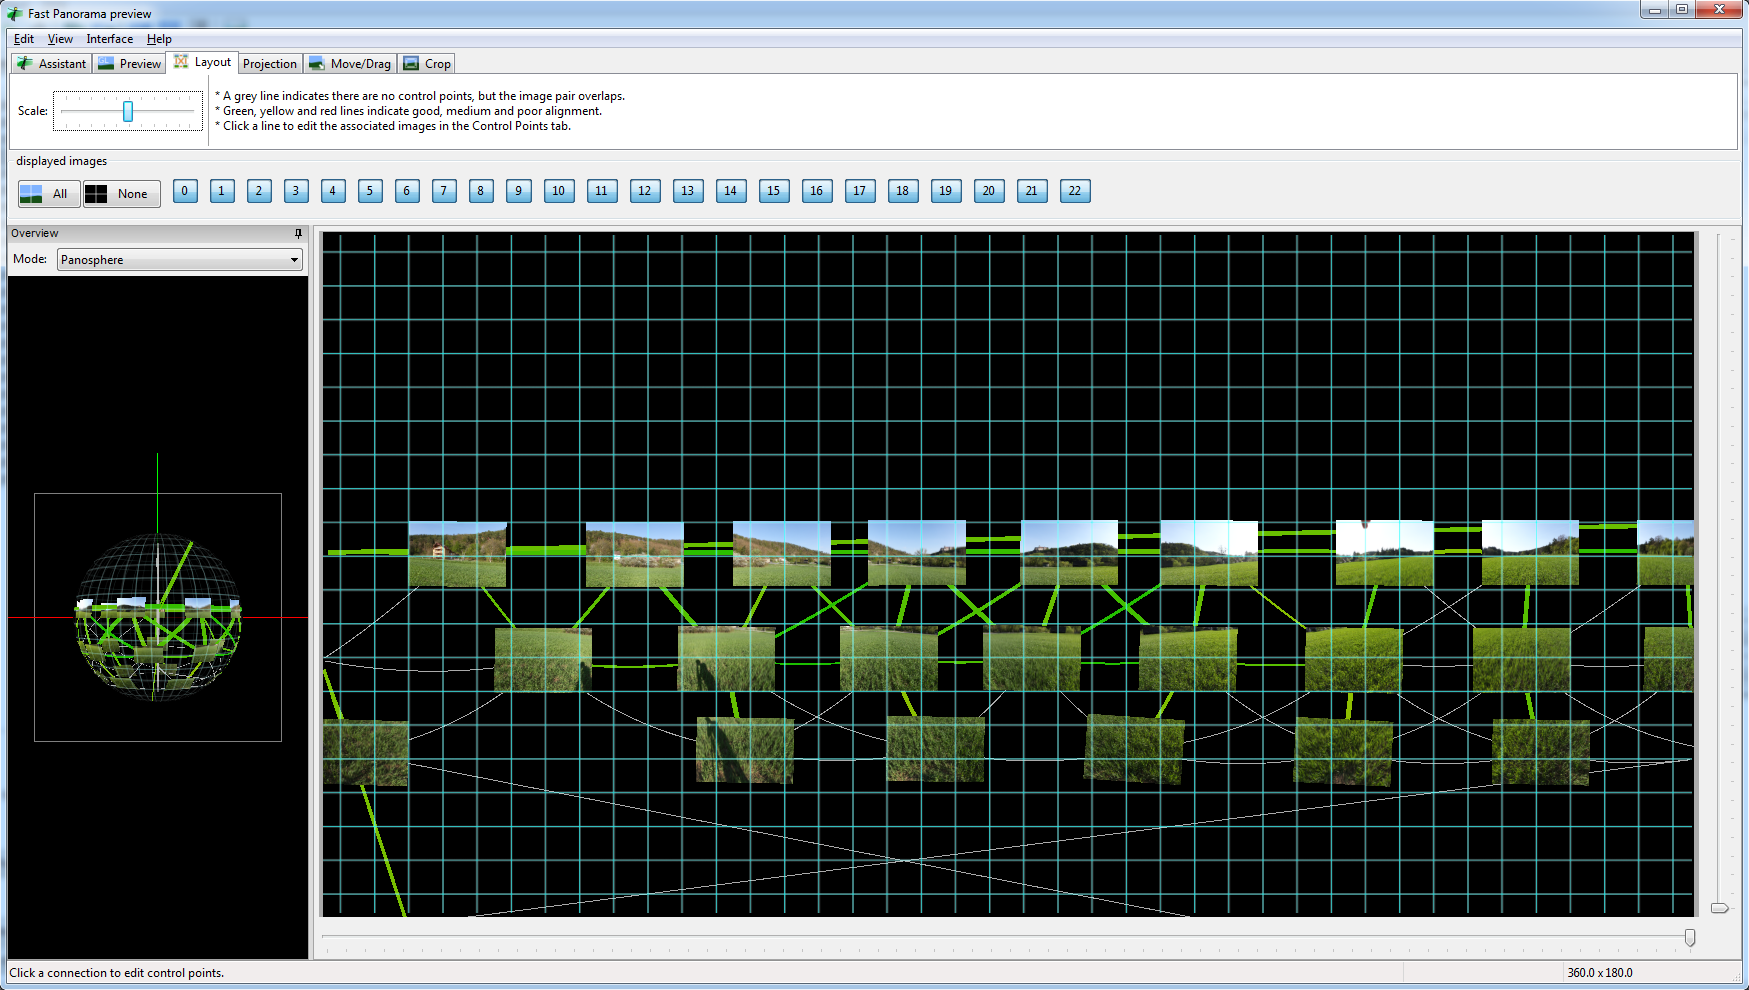
\includegraphics[width=\textwidth]{FastPreview.png}
    \caption{H\program{ugin}'s Fast Panorama Preview can be used to check which
      images are connected to its neighbours. Most important are good
      matches along the horizon, the images in the lower rows are
      clearly less important. If captured on a tripod, they should
      still match. }
  \label{fig:FastPanoPreview}
\end{figure}


\noindent
\colorbox{light-gray}{\fbox{\parbox[t]{0.975\linewidth}{
Basic rules to observe (use obvious inverses). 
%%%%%%%%%%%%%%%%%%%%%%%%%% DOUBLE-CHECK AGAIN!!!
\begin{itemize}
\item If image aligns well in azimuth but overshoots the grid to the
  right: Increase yaw accordingly (0.022°/pixel if image is 16384 pixels wide).
\item If the north end (left and right borders) is higher than the
  southern contact point: Increase pitch angle.
\item If north and south points are OK, but the western (right) half is
  higher than the eastern (left) half: Increase Roll angle.
\end{itemize}
The corrections required for pitch and roll may be surprisingly small!
}}}




Within a few rounds of adjustments, panorama creation, adding as layer
in the image editor, and comparing to the reference data, you should
achieve a match to fit your needs.

In case you have taken photographs in several rings but without a panorama tripod, you may have to
first align only the horizontal images (deselect the lower images to
exclude from optimisation), and when the horizon ring is aligned
perfectly, deactivate further optimisation in \program{Hugin} for those photos
while ``attaching'' (optimising) the lower photos. In \program{Hugin}'s \menu{Photos} tab,
select \menu{Optimise> Geometric> Custom Parameters}. This opens an
extra tab \menu{Optimiser}, where you can fine-tune your needs: Switch
off all variables for the photos in the horizon ring, and make sure
the lower photos fit in the preview after optimisation.

It may even help to define that the lower rows have been taken with a
different Lens, so the field of view and distortion settings of the
horizon row will be used as it had been found during the horizon-only
match.

By now you should have
enough experience what level of error may be acceptable for you.


\subsection{Artificial Panoramas}
\label{sec:landscapes:Artificial}

I have created a
website\footnote{\url{http://homepage.univie.ac.at/Georg.Zotti/php/panoCam.php}} where
you can enter geographical coordinates and download a file
\file{pano.kml}  which helps with image creation from \program{Google Earth}
imagery. Store this file for a site, let us call it
\landscape{MYPLACE}, into a new directory \file{GE\_MYPLACE} inside
your \file{landscapes} directory.

Store all scenes visible from the respective viewpoint
\landscape{MYPLACE} as picture into one common folder in your
\file{landscapes/GE\_MYPLACE} under the viewpoint name, e.g.,
\file{75-30.jpg}, which means 75 degrees from Nadir, azimuth 30
degrees.  Also, double-click the pano entry or the marker in \program{Google Earth} to open a window with the
basic content of your \file{landscape.ini}. Copy and paste from there
into a new file \file{landscape.ini} and adjust the obvious
entries. Complete as required with the entries described in
section~\ref{sec:landscapes:Spherical}.

On loading of the images, Hugin will not be able to detect any EXIF
lens data and ask you for the horizontal field of view. Enter 60
degrees, which is the standard value for \program{Google Earth}
screenshots\footnote{Note that if you work with \program{Google Earth Pro}, you
  can create different FoV!}.

The viewpoint names translate almost directly to the yaw and pitch
angles which you can enter in the image list in \program{Hugin}'s
\menu{Photos} tab. For example, switch to the \menu{Positions} display
on the right window edge in the \menu{Photo} tab, mark all images that
start with \file{25-} and assign a pitch angle of
$-90+\mathbf{25}=-65$. The second part of the names is directly the
azimuth.  In this case, don't run the optimizer, but you can
immediately set an output resolution and stitch
(see~\ref{sec:landscapes:stitching}). To get rid of the image
decorations (compass etc), apply masks\footnote{There is a wide
  overlap in the images to allow generous trimming.}. Postprocessing
steps are the same as for photo-panoramas: make sky invisible, crop,
etc.

It is also interesting to switch on the 3D buildings layer before
creating the images. If temples or other buildings are accurate, this
will give an even closer approximation to what would be visible
on-site. Note however that not every building will be modelled in
usable quality, and that usually vegetation is not included in the 3D
buildings layer. Also, if you are too close to buildings, they may be
cut away by the \emph{near clipping plane} of the rendering.

These images, based on \program{Google Earth} imagery and the SRTM
topographic model, seem usable as \emph{first rough approximation} to
a photo-based or surveyed panorama. Note that it is definitely not
accurate enough for representing nearby horizon features or critically
important mountain peaks, and please note that Google has image
copyright which at least requires you to acknowledge when displaying
these pictures.

\subsection{Nightscape Layer}
\label{sec:landscapes:landscapes:Nightscape}

Since version 0.13, Stellarium can simulate artificial illumination,
like streetlamps, bright windows, or the skyglow over cities\cite{Zotti-Wuchterl:SEAC2014}. One way to
create this layer is to make 2 panorama series during the day and night
and process these in the same \program{Hugin} project to align those photos,
and then stitch two separate images by selecting either the daylight or the
nighttime shots. The night panorama has to be processed to remove
stars, airplanes, etc.

The other way is a simple layer overpainted in the image processing
program. As rough recommendation, use several layers to prepare this
feature:
\begin{itemize}
\item Put a semitransparent black layer over your daylight image, this
  helps you to place your painted pixels.
\item Paint windows, street lamps, signs, \ldots. You may apply a
  layer style to produce some glow.
\item To draw an impression of more light in the atmosphere (city
  skyglow), use a gradient with some brownish color. Generally the
  color depends on the appropriate mix of city lights (sodium, mercury
  vapour, etc.). Note that on the city outskirts a simple vertical
  gradient will not work, towards the city the horizon is much
  brighter. Use a huge but weak brush to make a more spotty sky.
\item Use the existing landscape as template for the layer mask for
  this gradient sky layer. (You want to hide skyglow by leaves in the
  foreground!)
\item If you want to add only a few lights to an \file{old\_style}
  landscape, you need to provide only the panels showing those
  lights. Just load a side panel for reference, place a new layer on
  top, and paint the lights on windows, lamps etc. There is no light
  option for the ground texture. This makes \file{old\_style}
  landscapes best suited for localized light pollution, not city
  skyglow.
\end{itemize}

The resulting image is then declared in the \var{maptex\_illum} line
of \file{landscape.ini}. Try also to balance the global strength of
light pollution with the \var{light\_pollution} key, and a probable
minimal brightness with the \var{minimal\_brightness} key.

Try to match the visual appearance, not necessarily what photographs
may have recorded. E.g., the \landscape{Grossmugl} sky shows horizon
glow mostly towards the city of Vienna, where long-time exposures may
already be saturated.

The possibilities seem limited only by your time and skills!

\section{Other recommended software}
\label{sec:landscapes:otherSoftware}

Here is a short collection of other useful programs for (panorama)
image manipulation and other tasks on Windows.


\subsection{IrfanView}
\label{sec:landscapes:IrfanView}

\program{IrfanView} is a free image viewer for Windows with many
options. It can show almost any image format, including several camera
RAW formats, in windowed and full-screen mode. It is definitely
preferrable over any image viewer built into Windows. Unfortunately
however, it has no panorama viewer function!

\subsection{FSPViewer}
\label{sec:landscapes:FSPViewer}

\program{FSPViewer}\footnote{Further details are available on its home
  page \url{http://www.fsoft.it/FSPViewer/}.} by Fulvio
Senore is an excellent panorama viewer for equirectanglar
images. Images centered along the horizon can be viewed directly,
while settings for images with different minimum and maximum angles,
as well as ``hotspots'' (similar to hyperlinks) which move to
neighboring panoramas, can be configured in an \file{.FSV} text file
like figure~\ref{fig:FSPexample}.


\begin{figure}[h]\centering
\begin{configfile}
ImageName=Horizon_Rosenburg.jpg
WindowTitle=Horizon_Rosenburg 
hFov=70 
#Formula: HP=100*(h/2-upper)/(lower-upper) in Hugin crop, or
#         HP=100*zeroRow/imgHeight 
HorizonPosition=33.8
\end{configfile}
\caption{FSP configuration file (example)}
\label{fig:FSPexample}
\end{figure}

\subsection{Clink}
\label{sec:landscapes:clink}

\program{Clink}\footnote{\url{http://mridgers.github.io/clink/}} is a command
line enhancement for Windows developed by Martin Ridgers. If you have
ever worked under a Linux \program{bash}-like command line, you will
easily feel that Windows' \program{cmd.exe} is extremely limited. \program{Clink}
provides several useful features, most notably a really usable
command-line completion. It is not essential for our tasks, but a
general improvement of usability of the Windows command line which
else has not caused me any trouble.

\subsection{Cygwin}
\label{sec:landscapes:cygwin}

Compared to Linux, the command line of Windows can be a humbling experience. None of
the wonderful helpers taken for granted on Linux are
available. \program{Cygwin}\footnote{\url{https://cygwin.com/index.html}}
provides a command line console with \program{bash} shell and all the
niceties like \program{make}, \program{awk}, \program{sed}, etc.\ which seem
essential for routine work.  If you are used to Linux tools, use
inline scripts in your \file{Makefile}s and need more than \program{Clink} can
offer, you should install \program{Cygwin}.

\subsection{GNUWin32}
\label{sec:landscapes:GNUwin32}

Alternative to \program{Cygwin}, several of those nice tools (\program{sed},
\program{awk} etc.) have also been made available as standalone commands
for Windows. If you don't need the inline scripting capabilities in
\file{Makefile}s which you would get from \program{Cygwin} but just want to call
\program{awk} or \program{sed} inside your \program{.BAT} scripts, maybe this is enough.


%%% Local Variables: 
%%% mode: latex
%%% TeX-master: "guide"
%%% End: 

